\chapter{Developer Manual}
This manual will go through the needed steps to get started on extending and further developing on OKSE. The first sections will go through how to set up the development environment. The rest of the sections will go through the different parts of the system and how you can extend them.

\section{Requirements and Setup}
The recommended setup, as noted below, is using IntelliJ IDEA\footnote{\url{https://www.jetbrains.com/idea/}} as the Java IDE. However, other IDEs that meet the requirements listed below, or a combination should suffice. 

\subsection{Requirements and dependencies}

\subsubsection{Java}
The minimum required major version of Java is 8, and we do recommend to use the latest minor release. As of the writing of this guide, update 31 is the latest, and the version which is used to compile the packaged version of OKSE that is bundled.

\subsubsection{Apache Maven}
The project source code, tests and dependency management is structured with Apache Maven\footnote{\url{https://maven.apache.org}}. Maven is used to fetch dependencies, run the tests and to build the final jar files. The minimum major version of Maven is 3 and any minor version from 3.0.5 and up can be used. However, the development team recommends the latest version. As of the time of this writing, the latest version is 3.3.3.

It is worth mentioning, that many of the popular IDE software for Java bundles Maven support and does not require it to be installed separately on the system.

\subsection{Recommended IDE}
The development team strongly recommends IntelliJ IDEA Ultimate\footnote{\url{https://www.jetbrains.com/idea/}} as the Integrated Development Environment. Note that the free Community edition should suffice, but its worth mentioning that the Ultimate edition has better support for frameworks like Spring and TestNG (test framework of choice), which is used for the web administration interface. Both Community and Ultimate edition comes bundled with Maven.

\subsection{Test Framework: TestNG}
The system has a lot of unit tests, and the test framework of choice is TestNG\footnote{\url{http://testng.org/doc/index.html}}. Any new features and expansions of the system should be accompanied by unit tests. Please refer to the TestNG documentation\footnote{\url{http://testng.org/doc/documentation-main.html}} on how to write tests that suits the expansions needs.

\subsection{IntelliJ setup}
As the user stands free to choose the IDE, the setup documentation will be fairly basic and it will be based on IntelliJ.

Prerequisites: IntelliJ is installed, an Internet connection and the source code is stored locally.

\begin{enumerate}
    \item Open IntelliJ
    \item Click "Import Project" or File -> "Import Project"
    \item Browse the file system and select the source code folder
    \item Choose "Import project from external model"
    \item Choose "Maven"
    \item Check "Import Maven projects automatically"
    \item Click Next
    \item no.ntnu.okse... should be selected, click Next
    \item Select 1.8 (if it is not available, click "+" and add it)
    \item Click Next
    \item Click Finish
\end{enumerate}

After the IntelliJ window is opened with the project, all the needed dependencies will be downloaded. After this is complete, the project setup is complete.

\section{Overview of components}

\subsection{Application}

The \verb!Application.java! file that resides in the root of the project is the main invocation point when starting the OKSE application. The main operations performed in this class are initializing the web admin console, and the CoreService instance, which in turn boot up more services.

The most important thing to note regarding this main class, is that it is also the class in which further extensions should be registered. Extending the application with additional core services is done through registering them to the CoreService via the \verb!registerCoreService()! method.

Extending the application with additional protocol support is done through use of the \verb!addProtocolServers()! method of the CoreService instance.

\subsection{Web Admin}

The OKSE administration console is run using the Spring framework, more exact the spring-boot\footnote{\ref{https://spring.io/guides/gs/rest-service/}} package, using Thymeleaf-templates\footnote{\url{http://www.thymeleaf.org}}. The main aspects of the Web Admin component are its models, controllers, templates and front-end JavaScript. 

\subsubsection{Backend}



\subsubsection{Frontend}

HAKLOEV PLZ

\subsection{CoreService}

The CoreService is the main part of the OKSE message translation and brokering system. It is responsible for booting and stopping the registered core services, such as those described in subsequent sections of this manual.

Additionally, the CoreService boots up registered ProtocolServers, which are described in their own section below. The CoreService is also responsible for gracefully shutting down registered ProtocolServers.

As with all the OKSE core services, the main CoreService extends the AbstractCoreService class. This class holds some common attributes that are needed, as well as defninitions of the abstract methods for \verb!init()!, \verb!boot()!, \verb!run()! and \verb!stop()! actions.

All the services are intended to follow the singleton pattern, which in our implementation uses static references. Thus, the remaining needed methods and fields for initialization and instanciation are not provided by the abstract superclass. They have to be implemented using a similar approach as described in the \ref{sec:common-patterns-used} and \ref{sec:adding-new-core-services} chapters.

An overview of the boot sequence of the main OKSE components is described in figure \ref{fig:boot-sequence}.


\begin{center}
  \begin{figure}[ht!]
    \makebox[\textwidth]{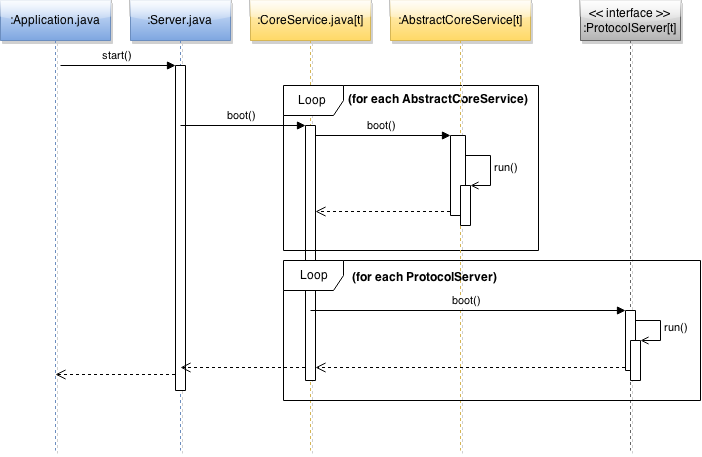
\includegraphics[width=\textwidth]{fig/bootSequence.png}}
    \caption{Boot sequence main components of OKSE}
    \label{fig:boot-sequence}
  \end{figure}
\end{center}

The details of the \verb!init()!, \verb!boot()! and \verb!run()! methods will vary from service to service, and protocol server to protocol server.

After the startup sequence has completed, all of the instances of either core services or protocol servers have their own dedicated thread that awaits the next task or event to execute.

\subsection{TopicService}

\subsection{SubscriptionService}

\subsection{MessageService}

\subsection{ProtocolServer}
 
\subsubsection{WSNotificationServer}

\subsubsection{AMQPServer}

\section{Common Patterns Used}
\label{sec:common-patterns-used}

\begin{itemize}
\item Singelton
\item ObserverPattern
\item Other: \begin{itemize}
\item Event Driven Single Service Single Thread
\end{itemize}
\end{itemize}

\section{Adding new protocols}

Something about AbstractProtocolServer class and ProtocolServer interface

\section{Adding new core services}
\label{sec:adding-new-core-services}

Something about AbstractCoreService, Singleton pattern and the needed methods to accomplish this, and the abstract methods needed from the superclass


\clearpage